\documentclass{article}
\usepackage{listings}
\usepackage{pdfpages}
\graphicspath{ {.} }

\usepackage{fancyhdr}
\usepackage[pdftex,
    pdfauthor={Aryan Gupta},
    pdftitle={ECGR4181 HW1 Report},
    pdfsubject={Homework Report},
    pdfkeywords={},
    pdfproducer={Latex with hyperref},
    pdfcreator={}
]{hyperref}
\usepackage[margin=1in]{geometry}
\hypersetup{colorlinks=true, linkcolor=black,urlcolor=black}
\usepackage[margin=1in]{geometry}
\usepackage{lastpage}
\usepackage[margin=1in]{geometry}
\usepackage{fancyhdr}
\usepackage{amsmath,amsfonts, amsthm}
\usepackage{float}
\usepackage{graphicx}

\lstset{
  basicstyle=\ttfamily,
  columns=fullflexible,
  frame=single,
  breaklines=true,
  postbreak=\mbox{$\hookrightarrow$\space},
}

\begin{document}
    \section{Dinero Simulator}
        The Dinero simulator is a cache simulator that lets the use experiment with different cache options such as associativity and block size. We modified various options to determine how it affects the cache miss ratio. The 12 main options given to us to test out are listed below.
        \begin{itemize}
            \item Split cache with 8Byte blocks directly mapped
            \item Split cache with 8Byte blocks 4 way associative
            \item Split cache with 32Byte blocks directly mapped
            \item Split cache with 32Byte blocks 4 way associative
            \item Split cache with 128Byte blocks directly mapped
            \item Split cache with 128Byte blocks 4 way associative
            \item Unified cache with 8Byte blocks directly mapped
            \item Unified cache with 8Byte blocks 4 way associative
            \item Unified cache with 32Byte blocks directly mapped
            \item Unified cache with 32Byte blocks 4 way associative
            \item Unified cache with 128Byte blocks directly mapped
            \item Unified cache with 128Byte blocks 4 way associative
        \end{itemize}
        The split caches were comprised of 16KB instruction cache and 16KB data cache. The unified caches were 32KB large. These experiments were ran using this command for split cache.
        \begin{lstlisting}
cat ../../project/trace.din | ./dineroIV -l1-dsize <DATA_CACHE_SIZE> -l1-dbsize <DATA_BLOCK_SIZE> -l1-dassoc <DATA_ASSOC> -l1-isize <INS_CACHE_SIZE> -l1-ibsize <INS_BLOCK_SIZE> -l1-iassoc <INS_ASSOC> -informatd
        \end{lstlisting}
        And this command for unified cache.
        \begin{lstlisting}
cat ../../project/trace.din | ./dineroIV -l1-usize <CACHE_SIZE> -l1-ubsize <BLOCK_SIZE> -l1-uassoc <DATA_ASSOC> -informatd
        \end{lstlisting}
        \par
        The result of the experiment with the dineroIV simulator was consistent with the theory taught in class. The results are laid neatly in this graph below.
        \begin{figure}[H]
            \centering
            \label{fig:uniMetric}
            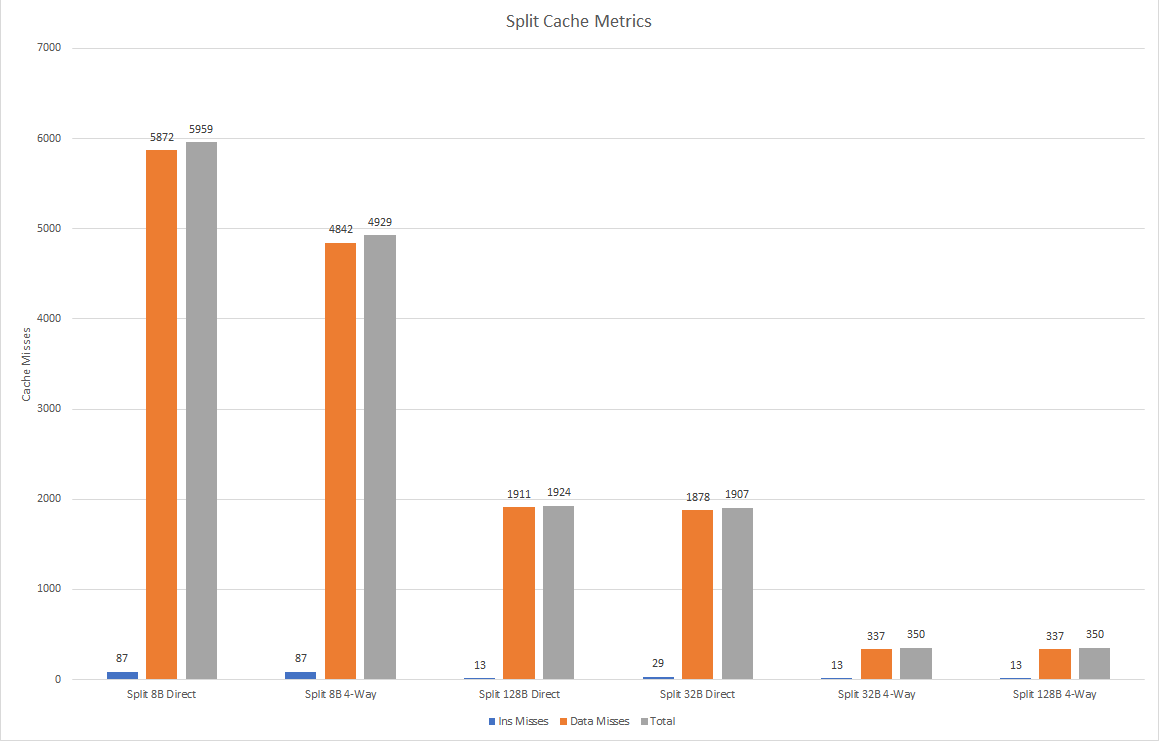
\includegraphics[width=\textwidth]{uni-cache-metrics.png}
            \caption{Metrics of a unified cache}
        \end{figure}
        A general trend that can be seen in Figure \ref{fig:uniMetric} is that as the associativity increases the miss rate drops. This is because when the associativity is increased a cache line is less likely to fight another line for a spot in the cache. This type of cache miss is known as conflict misses because 2 lines are conflicting for a spot in the cache. Another trend that can be seen is that as the size of the cache line is increased, the miss rate drops. This is because as the cache line size is increased the special locality of that line is also increased. When data is accessed, it is highly likely that some data next to or around that data will be accessed next or in the near future. By increasing the block size, we can take advantage of this fact and load possible future memory access into the cache before they are actually accessed. This type of cache is usually used in L2 caches because the data and instructions don’t need to be separated.
        \par
        Contrary to the L2 cache, the L1 cache is usually split by the data and instructions. This means that there are 2 "caches", one for the instructions and another one for data. This can benefit drastically because the way instructions are accessed is very different from the way data is accessed. Instructions have a lot more spatial locality and Data have more temporal locality. Figure \ref{fig:splitMetric} is a graph representing the metrics of the split cache.
        \begin{figure}[H]
            \label{fig:splitMetric}
            \begin{center}
                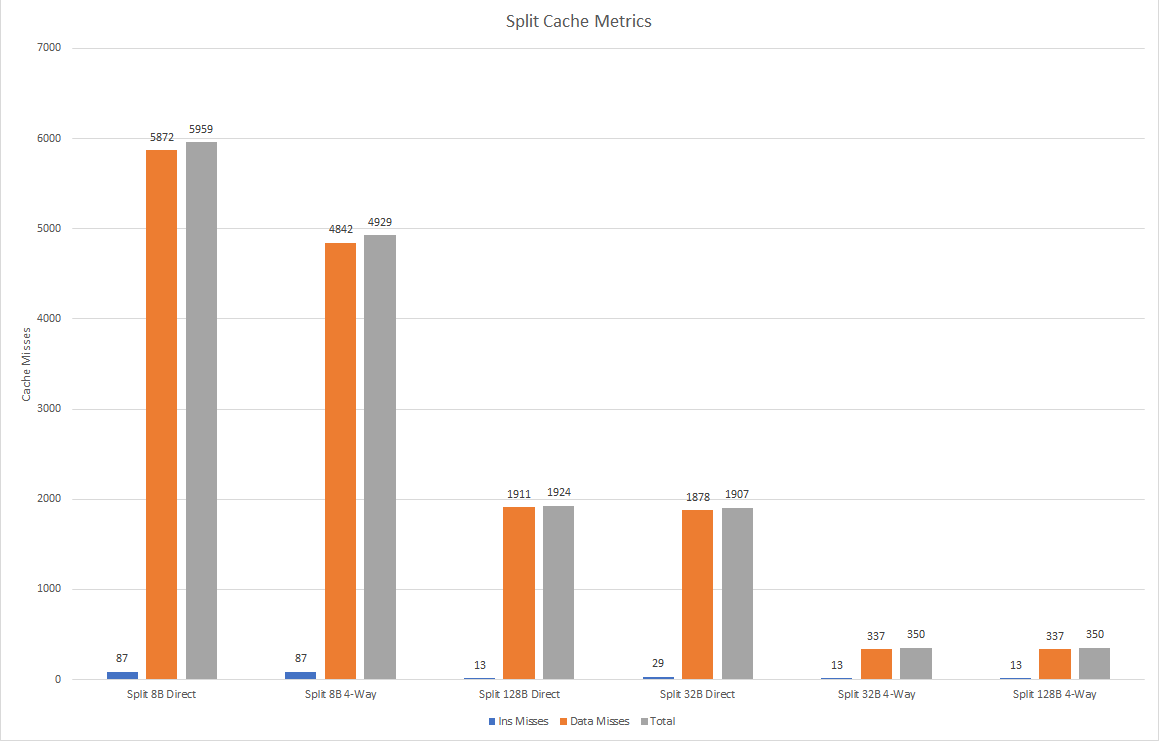
\includegraphics[width=\textwidth]{spl-cache-metrics.png}
                \caption{Metrics of a unified cache}
            \end{center}
        \end{figure}
        The graph plainly represents a decrease in cache misses as the associativity and cache block sizes are increased. These results are in line with the theory learned in class.
        \par
        Figure \ref{fig:diffMetric} shows the difference between using a split cache and a unified cache. There does not seem to be any clear pattern between using a split or unified cache. More experimentation is needed before anything concrete can be deducted.
        \begin{figure}[H]
            \label{fig:diffMetric}
            \begin{center}
                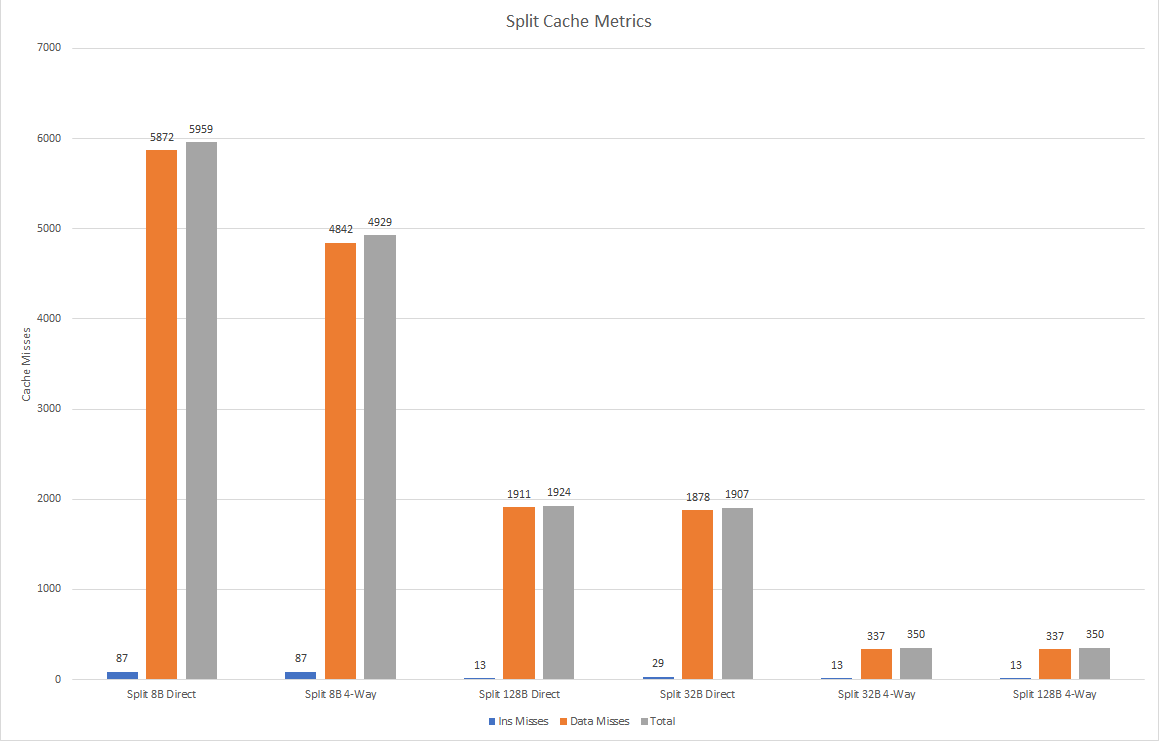
\includegraphics[width=\textwidth]{spl-cache-metrics.png}
                \caption{Metrics of a unified cache}
            \end{center}
        \end{figure}

    \subsection{Custom Cache Simulator}
        For part 2 of the assignment, we created our own Simulator similar to dineroIV. The code for this project is located in the \verb|src/| directory. I am using Arch Linux and I recognize that older systems may not support all the features used in the build system. I have tried as much as I could to add legacy support for older build systems. I was able to compile using gcc version 5 without any issues. In case you aren’t able to build the code, there is a prebuild binary in the \verb|bin/| directory named \verb|main.out|. To rebuild the binary, please run \verb|~$ make all| or just \verb|~$ make|.
        \subsubsection{The Code}
            The code consists of these classes
            \begin{itemize}
                \item Simulator
                \item Cache
                \item parse
                \item printer
            \end{itemize}
            The Simulator class is responsible for running the simulator. The c'tor of the class takes in the instructions to execute and parsed data from the command line. Using this information, the Simulator sets up the hierarchy of cache and then begins executing the instructions at the call of \verb|Simulator::simulate()|. Another member function: \verb|Simulator::getRatio()| returns the ratio of hits to the total number of access.
            \par
            The Cache class is where all the magic happens. The Cache class holds the addresses of the data that is currently in the cache. Because of associativity and the various other simulator options, there is also a valid bit and a Least Recently Used (lru) number. These 3 data members are grouped into a c-style struct called \verb|cache-info|. The lru bits will be discussed in greater detail later. Upon the construction of the Cache class, another c-style struct is created that defines which parts of the address are the tag, index, or offset. This simplifies the extraction of these bits during computation. An example is shown below.
            \begin{center}
            \begin{verbatim}
                        0x25F287AB
                        0b10010111110010  100001111010  1011
                          ~~~~~~~~~~~~~~  ~~~~~~~~~~~~  ~~~~
                                Tag           Index    Offset
            \end{verbatim}
            \end{center}
            In this example, the block-size is 16B and the Cache is 64KB. The offset bits are easy and can be calculated by using this equation.
            \[ Offset Bits = log_2(blocksize) = log_2(16) = 4  \]
            The Index bits can be calcuated by taking the cache size (64KB) and dividing it by the block-size.
            \[ Index Bits = log_2\left(\frac{cachesize}{blocksize}\right) = log_2\left(\frac{64KB}{16B}\right) = log_2\left(\frac{65536}{16}\right) = 12 \]
            The rest of the 32 bits are the tag.
            \[ Tag bits = 32 - blockbits - cachesize = 32 - 4 - 12 = 16 \]
            Using these 3 pieces of information, the masks and bit shifts can be calculated to extract each part of the address. More details can be viewed in \verb|Cache::getTag(ptr_t)|. Once the cache sizes and address bits are set, the replace and locate function are computed.
            \par
            The simulator goes through each of the instructions and depending if its a read, write, or a fetch, it calls the respective function. The Simulator has 2 \verb|Cache*| objects, one for the data and another for the instruction cache. When the simulator is run for a unified cache, the pointers point to one cache object. Each cache objects holds the number of cache misses and hits and can be queried by \verb|Cache::getHits() const| and \verb|Cache::getAccess() const|
            \par
            The other 2 files: \verb|parse| and \verb|printer| is responsible for parsing and printing various information to the console.
        \subsubsection{Running the Code}
            The code can be run in 2 ways. It can be run using lines from a file.
            \begin{lstlisting}
./bin/main.out -ftest/dry_trace.din --ucache-size=32K --ublock-size=128 --uassociativity=1
            \end{lstlisting}
            or from stdin
            \begin{lstlisting}
cat test/dry_trace.din | ./bin/main.out - --ucache-size=32K --ublock-size=128 --uassociativity=1
            \end{lstlisting}
            The program can be also run for a split cache by using
            \begin{lstlisting}
cat test/dry_trace.din | ./bin/main.out - --ucache-size=32K --ublock-size=128 --uassociativity=1
            \end{lstlisting}

    \subsection{Pintools}
        Pin tools was a very finicky software, trying to understand how it worked was very difficult until I had to ask a few of my friends that did get it working. From what we understood, pin is a program that queries information from the processor, the type of information it queries can be changed by the \verb|-t| command line argument. This argument takes in a dynamic library that queries the processor. In our test we used the \verb|allcache.so| library that shows cache information. The LINPAC benchmarks I was using were all precompiled, I could not find a source online that was viable for me to use. The Dhrystone benchmark has never worked for me, even with HW0. I’ve tried multiple sources and they don’t seem to give correct results. For example, Figure \ref{fig:dry_graph} shows me that no matter what optimization I use, I always get the same amount of cache misses in each level. Because some of the data is not easy to see in the graph I have also included Table \ref{fig:dry_table}. You can see that as the optimization level increases, the cache misses should go down as the optimization probably tries to reorder instructions to minimize the memory access.
        \begin{figure}[H]
            \label{fig:dry_graph}
            \begin{center}
                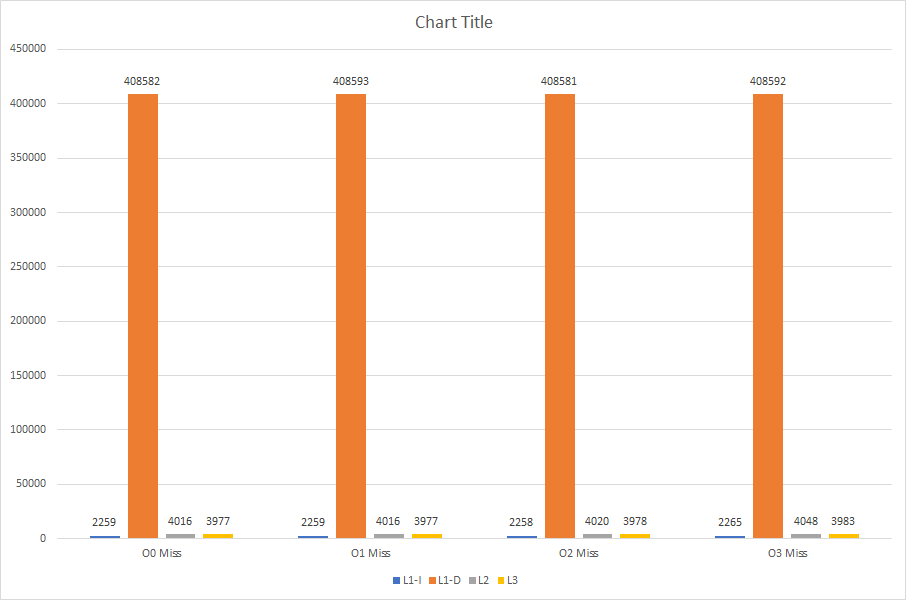
\includegraphics[width=\textwidth]{dry_graph.png}
                \caption{Metrics of a unified cache}
            \end{center}
        \end{figure}
        \begin{figure}[H]
            \label{fig:dry_table}
            \begin{center}
                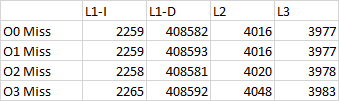
\includegraphics[width=\textwidth]{dry_table.png}
                \caption{Metrics of a unified cache}
            \end{center}
        \end{figure}

        % TODO HERE

    \subsection{Benchmark Memory Trace}
        The last part of the assignment was to create our own memory trace for dineroIV and use it on our cache simulator. One of the difficult parts was that all my machines were 64bit machines, so running pin tools to create a trace would create 64-bit addresses. The code that I wrote only works with 32-bit. After a bit of modification, I got it to work with 64-bit address. I could not get LINPAC to work with pin tools, I kept getting a segmentation fault. Here are the results for the Dhrystone trace.
        \begin{figure}[H]
            \label{fig:custom_dry}
            \begin{center}
                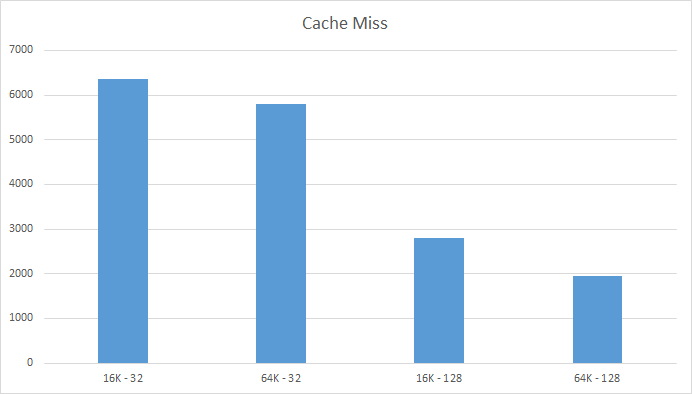
\includegraphics[width=\textwidth]{custom_dry.png}
                \caption{Dhrystone trace on custom cache simulator}
            \end{center}
        \end{figure}
        As you can see in this image, as we increase the block size, our cache misses go down. This is because of special locality in the program. When we address one location, it is highly likely that we will address another address in close vicinity. Another trend we can see is very similar to the previous one. When we increase the cache to a 64K cache then the cache misses drop, however not as sharply as the block size increase did. The decrease in Cache misses is because of the reduction in Capacity misses. Capacity misses are when our cache is full and we need to eject old data that we will need to fit in the new block.

\end{document}

